\section{Introduction}
The system in study was proposed by O.E. R\"ossler  in 1976, as a simplified model with shape and behavior similar to spirals in Lorenz system, which was not fully understood at the time due to the techniques known to study oscillators were not applicable to Lorenz model \cite{rossler1976equation}. The R\"ossler equations are:

\begin{equation}
	\begin{array}{ll}
            \dot{x}&=-y-z\\
            \dot{y}&=x+ay\\
            \dot{z}&=b+z\left(x-c\right)
    \end{array}
\end{equation}

Although R\"ossler affirmed that the system did not have immediate physical interpretation \cite{rossler1976equation}, nowadays some applications can be found using the model as a mechanism and not as an abstraction of a physical system. The model presented has been used as a tool for image cryptography as it was shown by Mandal \textit{et al.} in  \cite{mandal2014symmetric}; in further work, Laiphrakpam and Khumanthem proposed improvements to Mandal's algorithm, as it is shown in \cite{laiphrakpam2017cryptanalysis}. On the other hand, coupled R\"ossler system with different inputs have been used to measure the correlation of time series, as Weule \textit{et al.} showed in \cite{weule1998detection}.

In order to bring the system to the real world, R\"ossler equations can be represented by a circuit, as Canals \textit{et al.} show in \cite{canals2014random}. The proposed circuit is shown in Fig. \ref{fig:circuito} and can be translated to 
\begin{equation}
	\begin{array}{ll}
            RC\dot{x}&=-y-z\\
            RC\dot{y}&=x+ay\\
            RC\dot{z}&=b+z\left(x-c\right)
    \end{array}\quad\quad\begin{array}{ll}
            a &= \dfrac{100k\Omega}{R_a}\vspace{2.5mm}\\
            b &= V_{cc}\dfrac{100k\Omega}{R_b}\vspace{2.5mm}\\
            c &= \dfrac{100k\Omega}{R_c}
    \end{array}\label{eq:circ}
\end{equation}
In \cite{canals2014random} they use this circuit to generate true random numbers using the output of the voltage of the node $z$. The nodes $x$ and $y$ have a fixed frequency of oscillation if the other variable is set to 0, since their rate of change are linear. In contrast, $z$ induces chaos to the circuit, due to its nonlinear behavior. In this manner, this variable was selected to be the output as its chaotic behavior is useful to generate random numbers \cite{canals2014random}.

Therefore, in this paper will study the question: ``Which interval of values for the supplied voltages and resistances in the circuit can preserve the chaos of the system?''. It is conjectured that with small values of the resistance, the system will reach their maximum charge quicker than the simulation period, therefore it will stabilize and won't show chaotic behaviour. Otherwise, with the voltages supplied by the battery, it is hypothesized that for larger values the circuit would reach the maximum charge quicker so it will not be chaotic either.

In order to answer this question, the system will be simulated with different types of inputs, so it can be analyzed how the circuit behaves if the battery supplies different voltages to the system. Lastly, two parameters will be changed so it can be observed how the system acts with different resistance values, in order to find a interval where the system still has chaotic behaviour.

In section \ref{sec:meth}, the dynamic equation can be found, as well as the numerical algorithms to simulate the system. In section \ref{sec:result}, the results of the simulations with different types of inputs and parameters. In section \ref{sec:resultAn}, the analysis of the obtained results and their justification. Lastly, the conclusions of the work are presented in section \ref{sec:conc}.

\section{Methods}\label{sec:meth}
\subsection{Dynamic System}
In the circuit presented, according to Canals \textit{et al.} \cite{canals2014random}, the variables $x$, $y$ and $z$ represent the voltages through the nodes shown in Fig. \ref{fig:circuito}. The $RC$ parameter defines the system's time (in seconds), the supplied voltages are $V_{cc}=15V$ and $V_{ss}=-15V$; $R_a$, $R_b$ y $R_c$ are resistors in $k\Omega$ used to calculate the system's original parameters, as shown in (\ref{eq:circ}).
\begin{figure*}
    \centering
    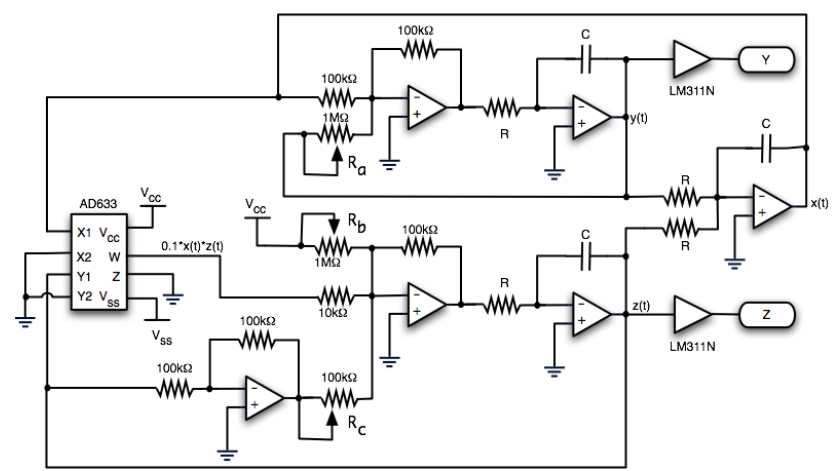
\includegraphics[scale=0.325]{figs/Circuito.png}
    \caption{R\"ossler circuit representation \cite{canals2014random}.}
    \label{fig:circuito}
\end{figure*}
In order to simulate the system in Simulink, the state and output equations will be used; thus, the dynamic equation is given by
\begin{equation}
\begin{cases}
	\dot{x_1}=\dfrac{1}{RC}\left(-x_2-y\right)&\vspace{2mm}\\\vspace{2mm}
	\dot{x_2}=\dfrac{1}{RC}\left(x_1+\dfrac{100k\Omega}{R_a}x_2\right)&\\
	\dot{x_3}=\dfrac{1}{RC}\left[\left(V_{cc0}+u\left(t\right)\right)\dfrac{100k\Omega}{R_b}+y\left(x_1-\dfrac{100k\Omega}{R_c}\right)\right]&\\
	y = x_3
\end{cases}
\label{eq:state}
\end{equation}
where $y$ is the output and $u$ the input; note that the parameter $V_{cc}$ was selected as input, thus we select an initial value $V_{cc0}$ and add the input $u\left(t\right)$ in Volts. For the rest of this document, the state variable $x_3$ will be referred as $y$, since it has been chosen as the output.

\subsection{Implementation using Simulink}
Using equation system (\ref{eq:state}), a simulation diagram was constructed using Simulink, as Fig. \ref{fig:simulink}
shows.
\begin{figure}[H]
    \centering
    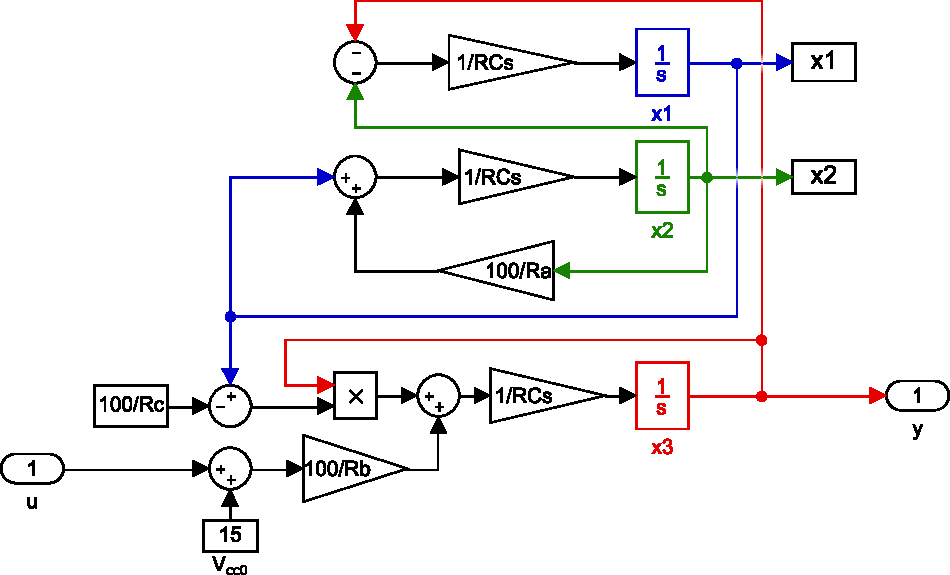
\includegraphics[scale=0.55]{figs/simulink.pdf}
    \caption{Simulation diagram for R\"ossler system.}
    \label{fig:simulink}
\end{figure}

\subsection{Numerical algorithms}
	Given the differential equation to solve:
    \begin{equation}
        \dot{x} = f\left(t,x\right)
    \end{equation}
    With the initial condition $x\left(0\right)=x_0$ and a step of time $h$ that discretize the system. The simulation for the solution of $x$ can be obtained with different methods such as Runge-kutta and Euler. This algorithms and more can be found in \cite{kutta}. Note that the following methods will have implicit sample time.
    
    \subsubsection{Euler}
    Using Euler's method, the difference equation is:
    \begin{equation}
        x\left(k+1\right) = x\left(k\right) + hf\left(k,x\left(k\right)\right)
    \end{equation}
    
    \subsubsection{Runge-kutta}
    In the fourth order Runge-Kutta's method, the difference equation is:
    \begin{equation}
        x\left(k+1\right) = x\left(k\right) + \dfrac{h}{6}\left(k_1 + 2k_2 + 2k_3 + k_4\right)
    \end{equation}
    Where:
    \begin{equation}
	\begin{array}{ll}
        k_1 = f\left(k, x\left(k\right)\right)\vspace{1mm} \\
        k_2 = f\left(k + \dfrac{h}{2}, x\left(k\right) + \dfrac{hk_1}{2}\right)\vspace{1mm} \\
        k_3 = f\left(k + \dfrac{h}{2}, x\left(k\right) + \dfrac{hk_2}{2}\right)\vspace{1mm} \\
        k_4 = f\left(k + h, x\left(k\right) + hk_3\right)
    \end{array}
    \end{equation}
    
    For the system in study, the difference equations are:
    
    \begin{equation}
        \mathds{X}\left(j+1\right) = \mathds{X}(j) + \dfrac{h}{6}\left(\mathds{K}_1 + 2\mathds{K}_2 + 2\mathds{K}_3 + \mathds{K}_4\right)
    \end{equation}
    Where: \[\mathds{X}(j)=\left[x_1(j)\quad x_2(j)\quad y(j)\right]^T\quad\mathds{K}_i=\left[k_{ix_1}\quad k_{ix_2}\quad k_{iy}\right]^T\]
    Then, we have:
    \setlength{\arraycolsep}{0.0em}
    \begin{eqnarray}
    k_{1x_1}(j)&=& -x_2(j) - y(j)\nonumber\\
    k_{1x_2}(j)&=& x_1(j) + \dfrac{100}{R_a}x_2(j)\nonumber\\
    k_{1y}(j)&=& [V_{cc0}+u(j)]\dfrac{100}{R_b} + \left(x_1(j) - \dfrac{100}{R_c}\right)y(j)\nonumber
    \end{eqnarray}
    \begin{eqnarray}
    k_{2x_1}(j)&=&-\left(x_2(j) + \dfrac{hk_{1x_1}(j)}{2}\right) - \left(y(j) + \dfrac{hk_{1x_1}(j)}{2}\right)\nonumber\\
    k_{2x_2}(j)&=& \left(x_1(j) + \dfrac{hk_{1x_2}(j)}{2}\right) + \dfrac{100}{R_a}\left(x_2(j) + \dfrac{hk_{1x_2}(j)}{2}\right)\nonumber\\
    k_{2y(j)}&=&[V_{cc0}+u(j)]\dfrac{100}{R_b}\nonumber\\
    &&+ \left[\left(x_1(j) + \dfrac{hk_{1y}(j)}{2}\right) - \dfrac{100}{R_c}\right]\left(y(j) + \dfrac{hk_{1y}(j)}{2}\right)\nonumber
    \end{eqnarray}
    \begin{eqnarray}
    k_{3x_1}(j)&=&-\left(x_2(j) + \dfrac{hk_{2x_1}(j)}{2}\right) - \left(y(j) + \dfrac{hk_{2x_1}(j)}{2}\right)\nonumber\\
    k_{3x_2}(j)&=& \left(x_1(j) + \dfrac{hk_{2x_2}(j)}{2}\right) + \dfrac{100}{R_a}\left(x_2(j) + \dfrac{hk_{2x_2}(j)}{2}\right)\nonumber\\
    k_{3y}(j)&=&[V_{cc0}+u(j)]\dfrac{100}{R_b} \nonumber\\
    &&+ \left[\left(x_1(j) + \dfrac{hk_{2y}(j)}{2}\right) - \dfrac{100}{R_c}\right]\left(y(j) + \dfrac{hk_{2y}(j)}{2}\right)\nonumber
    \end{eqnarray}
    \begin{eqnarray}
    k_{4x_1}(j)&=&-\left(x_2(j) + hk_{3x_1}(j)\right) - \left(y(j) + hk_{3x_1}(j)\right)\nonumber\\
    k_{4x_2}(j)&=&\left(x_1(j) + hk_{3x_2}\right) + \dfrac{100}{R_a}\left(x_2(j) + hk_{3x_2}\right)\nonumber\\
    k_{4y}(j)&=&[V_{cc0}+u(j)]\dfrac{100}{R_b} \nonumber\\
    &&+ \left[\left(x_1(j) + hk_{3y}\right) - \dfrac{100}{R_c}\right]\left(y(j) + hk_{3y}\right)\nonumber
\end{eqnarray}
\setlength{\arraycolsep}{5pt}
